%% ================================================================================
%% This LaTeX file was created by AbiWord.                                         
%% AbiWord is a free, Open Source word processor.                                  
%% More information about AbiWord is available at http://www.abisource.com/        
%% ================================================================================

\documentclass[a4paper,portrait,12pt]{article}
\usepackage[latin1]{inputenc}
\usepackage{calc}
\usepackage{setspace}
\usepackage{fixltx2e}
\usepackage{graphicx}
\usepackage{multicol}
\usepackage{minted}
\usepackage{listings}
\usepackage{algorithmicx}
\usepackage{algpseudocode}
% \usepackage{csquotes}
%\usepackage[normalem]{ulem}
%% Please revise the following command, if your babel
%% package does not support en-US
%\usepackage{babel}
\usepackage{color}
\usepackage{hyperref}
 
\begin{document}

\setlength{\oddsidemargin}{0.9847in-1in}
\setlength{\textwidth}{\paperwidth - 0.9847in-0.9847in}

\author{Ovidiu Popoviciu, 2036725}
\date{17th November 2017}
\title{Twitter Event Detection - MSci}
\maketitle

%%%%%%%%%%%%%%%%%%%%%%%%%%%%%%%%%%%%%%%%%%%%%%%%%%%%%%%%%%%%%%%%%%%%%%%%%%%%%%%%%%
\section{Introduction}

Event detection in social media is a challenging task.
This is due to: 
\begin{itemize}
	\item The massive number of tweets (approx. 500 million tweets per day in 2016 \cite{tweetStats}).
	\item Amount of relevant tweets is very small (90\% are junk).
	\item Limitations with the API (until recently \cite{twitterPremium}).
	\item Importance of events and scalability issues.
	\item Spelling and grammar mistakes.
	\item Abbreviations and acronyms.
\end{itemize}

The objective of this work is to evaluate a stage of the event detection process initially defined by McMinn et al. \cite{McMinn2013} \cite{McMinn2015} on a collection of tweets.

%%%%%%%%%%%%%%%%%%%%%%%%%%%%%%%%%%%%%%%%%%%%%%%%%%%%%%%%%%%%%%%%%%%%%%%%%%%%%%%%%%
\section{Approach}
\cite{McMinn2013} \cite{McMinn2015}

Two approaches are defined, each executed after the clustering stage provided by McMinn et al. \cite{McMinn2013}.

Following the work of McMinn et al. \cite{McMinn2013}, the steps taken in the processing of the dataset are:
\begin{itemize}
	\item \textbf{Data collection} was already completed, and the dataset from the previous study shared for this experiment.
	\item \textbf{Pre-processing}. The dataset was already pre-processed. Tweets were parsed, tagged and filtered. All that remained were the relevant tweets with tokens that might relate back to an event.
	\item \textbf{Clustering}. The dataset contained clusters of tweets already defined, through the use of an Inverted Index and tweets were grouped using weight cosine similarity score.
	\item \textbf{Burst Detection}. Check for temporal bursts of a named entity in a window period of minutes to hours. This step was completed in conjunction with event merging.
	\item \textbf{Cluster Identification}. In McMinn et al. \cite{McMinn2013} evaluation program, clusters are already considered to map to a specific event since groups of tweets with no named entities have been removed.
	\item \textbf{Event Merging}. Merging events that have multiple named entities. Discussion of this work is focused on this step.
\end{itemize}

The dataset provided was pre-processed and organised into clusters.
The missing stages, provided in this work, are an enhancement to cluster identification and a different approach on event merging.
The two approaches are:
\begin{enumerate}
	\item Filtering.\\
	      \\
	      The goal was to identify clusters which have limited or no relevance to any significant events and to remove them.\\
	      \\
	      This step was an enhancement of Cluster Identification.
	      More specifically, the objective was to see whether removing clusters with a particular number of tweets might reduce the dataset, resulting in an increased precision of the system. \\
	      \\
	      The filtering step was simple, as it consisted of counting the number of tweets in each cluster, and dropping clusters with a size less than a number \textit{N}.
	      In this experiment, \textit{N} takes values from [5, 25].
	\item Merging. \\
	      \\
	      The goal was to study whether clusters with the same named entity, lying within the same temporal burst could be merged. \\
	      \\
		  In McMinn's study, clustering of tweets was optimised performance-wise by reducing the number of tweets retrieved from the Inverted Index and, thus, reducing the number of comparisons for each tweet.
	      Thus, the initial objective was to check whether multiple clusters with the same event (and same named entity) had been created within a specific time period and if merging of these clusters would have a positive effect on the performance of the system.\\
	      \\
	      Clusters with the same named identity residing in the same temporal window were merged.
	      The merge action was simply the addition of all tweets from the selected cluster to its named entity match.
	      Comparison of window temporality was executed using the difference between the centroid times of two clusters, where the centroid time is the mean of all the tweets in a cluster.\\

	      The computationally expensive section of this approach was that the previous array of clusters must had been kept sorted by time.
	      For each processed cluster, the first cluster to compare it against must be the most \"recent\" for this approach to bare fruit.
	      Thus, every time a new cluster got added to the \textit{previousCluster} array or the centroid time of a cluster was updated, then the array was re-sorted.\\
	      Fortunately, since only one cluster was updated at a time, the sort operation was computationally inexpensive (\textit{O}(\textit{N}) on nearly sorted array, using Bubble Sort.).

	      The window was tested with values (in minutes): 7, 15, 30, 60, 120 and 240.
	      \\\\
	      Pseudocode:
	      \begin{algorithmic}
		      \ForAll{$cluster$ of $clusters$}
		      \ForAll{$previous$ of $previousClusters$}
		      \If{$cluster.timestamp - previous.timestamp\geq window$}
		      \State $previousClusters.add(cluster)$
		      \State $break$
		      \EndIf
		      \If{$cluster.entity = previous.entity$}
		      \State $previous.addTweets(cluster.tweets)$
		      \State $break$
		      \EndIf
		      \EndFor
		      \State $previousClusters.sort()$
		      \EndFor
	      \end{algorithmic}
\end{enumerate}

The evaluation and discussion of the two approaches are dicusses in Section \ref{section-eval} and Section \ref{section-discussion}.

%%%%%%%%%%%%%%%%%%%%%%%%%%%%%%%%%%%%%%%%%%%%%%%%%%%%%%%%%%%%%%%%%%%%%%%%%%%%%%%%%%
\section{Code Description}
The implementation of the techniques were written in Java, due its object-oriented structure, efficiency and ability to handle 64-bit Integer values available from the dataset.

\begin{figure}[h!]
	\centering
	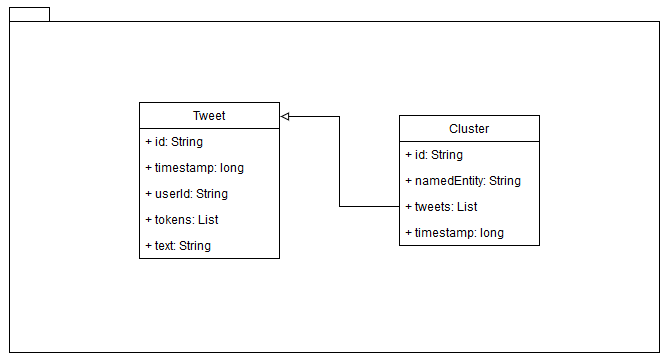
\includegraphics[width=0.5\linewidth]{images/modelUML.png}
	\caption{UML model classes}
	\label{fig:modelUML}
\end{figure}

Initially, two model classes were defined, as seen in Figure \ref{fig:modelUML}.
The first class, Tweet, contained the appropriate fields for identifying a tweet, such as: tweet ID, timestamp, user ID, parsed tweet tokens and the body text of the tweet.
Additionally, a second model class defined was Cluster. 
Cluster class contained a list of tweets with the same properties and was defined by a cluster ID, by the named entity identified by all the tweets and a timestamp which would hold the centroid time of all tweets in that specific cluster.\\

The data set was read from local disk through an instance of IOProcessor, which is an interface for reading data.
Since the data was in CSV format, CSVProcessor was a class that implemeted the IOProcessor interface.
It provided methods for reading CSV cluster files and instantiating model classes.
Diagram for Processor classes can be seen in Figure \ref{fig:processorUML}. \\

\begin{figure}[h!]
	\centering
	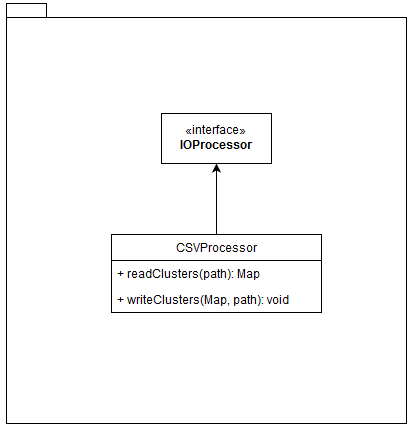
\includegraphics[width=0.5\linewidth]{images/processorUML.png}
	\caption{UML IO processor classes}
	\label{fig:processorUML}
\end{figure}

Data was read and processed as a stream of Cluster objects on which multiple sequential operations could be applied.
ClusterFilter was an interface that could be extended to add more operations.
The available operations, as seen in \ref{fig:filterUML}, are:
\begin{itemize}
	\item NumberOfTweetsFilter - was a class that filters the cluster by a set number of tweets.
	      A variable containing the number of tweets to filter by could be passed to the constructor of this class.
	\item MergeNamedEntityFilter - was a filter that merges clusters with the same named entities.
		  A variable denoting the time window could be initialized from the constructor of this class.
		  To speed up the performance of the filter, a map indexed by entities to list of clusters was used.
		  Every time a new cluster had to be processed, the list of groups with the same entity was retrieved from the map. 
		  This approach reduced the number of clusters to compare to.
		  However, it created a more complex data structure with the map of arrays.
		  In short, this approach traded off space complexity for time complexity. 

\end{itemize}

\begin{figure}[h!]
	\centering
	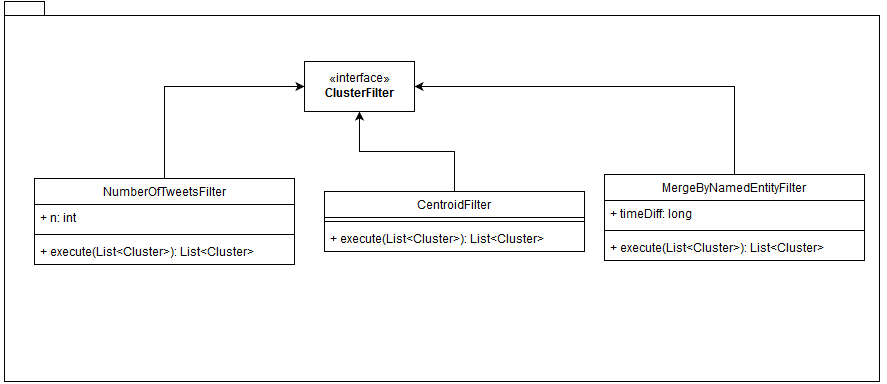
\includegraphics[width=0.7\linewidth]{images/filterUML.png}
	\caption{UML filter classes}
	\label{fig:filterUML}
\end{figure}

Each one of these filters could be applied in any sequence and the entire code could be run into a class containing the main function.
The Main class contained references to the other model, processor and filter classes and the entire flow of the system.
For the two approaches, two main classes were defined: \textit{MergeNamedEntities.java} and \textit{FilterByNumberOfTweets.java}.
The classes read data from IOProcessor, applied the filtering and merging operations on the stream of data and wrote the resulting clusters back to a new CSV file.

\begin{figure}[h!]
	\centering
	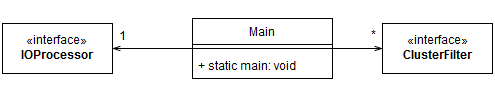
\includegraphics[width=0.7\linewidth]{images/mainUML.png}
	\caption{UML Main class}
	\label{fig:mainUML}
\end{figure}

The evaluation stage was the same as McMinn et al. \cite{McMinn2013}, which used a python script to evaluate the CSV files containing the clusters against crowd gathered events.
Additionally, due to the repetitive nature of the approaches, evaluating each CSV cluster file, gathering of results and manually pasting them into a data processor (e.g. Excel) might have taken a long time.
For this problem, Gradle tasks were implemented that automatically ran the two Java programs and generated all the files using only one command.
To gather the results from the output of the Python evaluation program, a NodeJS script was developed that ran the evaluation automatically and created a JSON containing the respective results.
As an example, all the results for the 1-day dataset with the filtering approach applied, would be contained within a single JSON file named \textit{1day-filtered.json}.
The JSON schema was defined as follows:

\begin{lstlisting}[caption=JSON Schema Example, label=json-schema]
[{
    "file": "0",
    "data": {
        "events": {
            "total": 506,
            "detected": 19
        },
        "clusters": {
            "total": 8829,
            "matched": 120
        },
        "stats": {
            "recall": 0.038,
            "precision": 0.014,
            "fmeasure": 0.02
        }
    }
},
...
]
\end{lstlisting}

The schema contained a number of properties, of which the most important were:
\begin{itemize}
	\item \textit{file} - this denoted the file that was used for evaluation.
	      For example, in the case of filtering approach, a file with the name \textit{8.csv} denoted that a filtering of a minimum number of 8 tweets had been applied to the initial dataset.
	\item \textit{data} - this property contained an object of the statistics of the evaluation.
\end{itemize}

The rest of the properties are self-descriptive.\\

Once all files had been evaluated, the JSON schemas were loaded into a JavaScript browser file.
This JavaScript file contained logic that constructs user-friendly visualizations of the results.
The charting functionality was provided by the frappe-charts package \cite{frappeCharts}.\\

The source code is available in the \textit{source} folder.
Instructions on how to run the code are contained in the \textit{README.md} file.

%%%%%%%%%%%%%%%%%%%%%%%%%%%%%%%%%%%%%%%%%%%%%%%%%%%%%%%%%%%%%%%%%%%%%%%%%%%%%%%%%%
\section{Evaluation}
\label{section-eval}

The evaluation of the two approaches relied on a few measures:
\begin{itemize}
	\item \textbf{Precision}.
	      This measure defines the proportion of the clusters that are relevant out of the returned set of events.
	\item \textbf{Recall}.
	      Defines the fraction of clusters that were found to be relevant out of the entire set of relevant events.
	      This measure, in theory, could not increase further than its baseline value, since it is largely dependent on the clustering step.
	\item \textbf{F-Measure}.
	      It is an overall score of performance, and is calculated as the weighted harmonic mean of the precision and recall measures.
\end{itemize}

Since recall precision cannot increase, then the evaluation focuses on increased precision with minimal negative impact to recall.
However, the results were surpring, as mentioned in the next paragraphs.\\
\\
Initially, the two baseline CSV files containing 1-day and 7-days data had been evaluated.
In the following figures, the element \textbf{0} on the \textit{x}-axis, is considered the baseline result.
The rest of the elements, could be considered in the context of either filtering or merging.
For example, the element \textbf{8} in the context of filtering, refers to the clusters which had been filtered by a minimum of 8 tweets.
Additionally, the element \textbf{30} in the context of merging, refers to the window value of 30 minutes.

A summary of the results, based on the f-measure for all sets can be seen in \ref{fig:summary}.
Additionally, the full results of the experiment can be viewed in Appendix \ref{appendix:results}.
An interactive visualisation of the results is available in the source code.
Instructions were provided within the source folder, in the \textit{README.md} file.

\begin{enumerate}
	\item \textbf{Filtering}\\
	\\
	      Filtering by number of tweets had a massive effect on the results of the evaluation. \\
	      By applying process on the 1-day data set, the precision increased by a magnitude while recall remained constant.
	      The change in precision might be due to junk clusters that had no relevance.
	      \begin{figure}[h!]
		      \centering
		      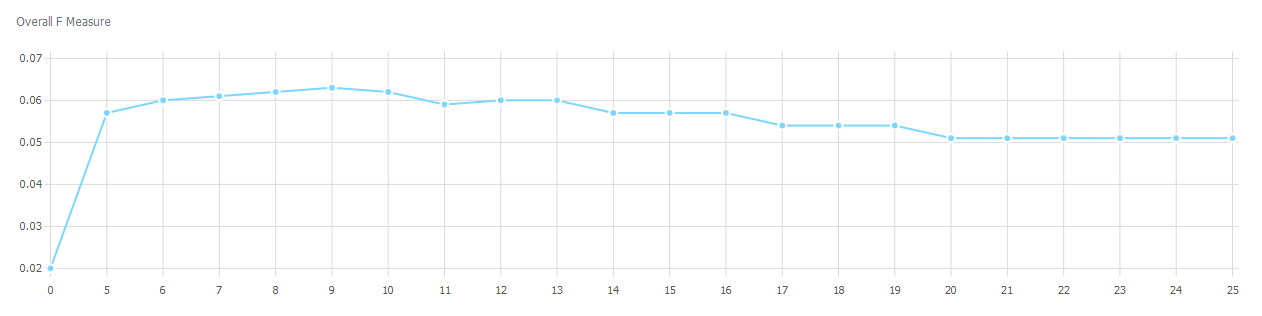
\includegraphics[width=\linewidth]{images/1day-filtered-f-measure.png}
		      \caption{1 Day Filtered - F-Measure}
		      \label{fig:1day-filtered-f-measure}
	      \end{figure}

	      As mentioned before, \textit{N} was tested within a range of [5, 25] and the results can be seen in Figure \ref{fig:1day-filtered-f-measure}.
	      The overall f-measure jumped from the initial evaluation and slowly increased up until \textit{N = 10}.
	      The f-measure slowly decreased thereafter, due to the number of relevant clusters being slowly filtered out.
	      This negatively impacted the recall measurement, from a base measure of 0.038 to 0.28.
	      On the other hand, precision increased dramatically as the number of clusters on each experiment decreased.
	      \\
	      Finally, for the 1-day data set, the optimal number of tweets in a cluster was 10.
	      This provided the highest f-measure of the entire range [5, 25] and with recall remaining constant.

	      Applying the same process on the 7-day data set, similar results emerged.
	      The overall f-measure jumped from the initial value of 0.026 to a maximum value of 0.242, for \textit{N = 11}.
	      Precision increased with incremental of \textit{N} while recall had slowly decreased, but with no major impact.
	      The trend of the f-measure for the 7-day data set can be seen in Figure \ref{fig:7days-filtered-f-measure}.
	      \begin{figure}[h!]
		      \centering
		      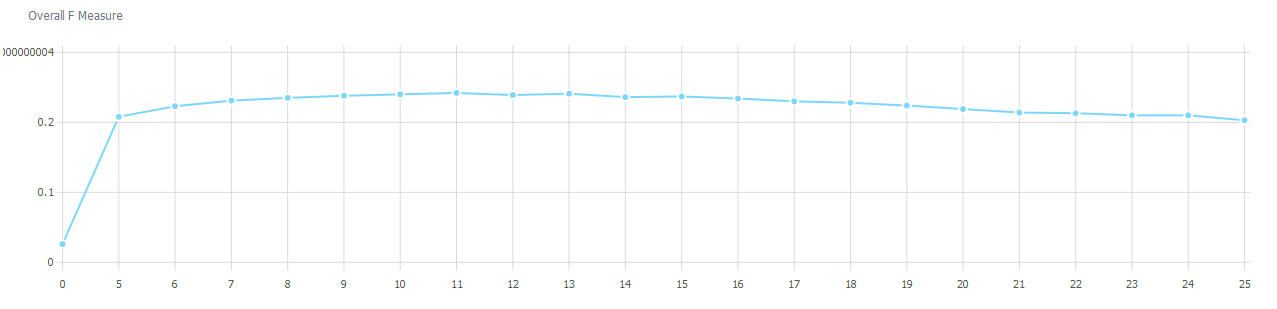
\includegraphics[width=\linewidth]{images/7days-filtered-f-measure.png}
		      \caption{7 Days Filtered - F-Measure}
		      \label{fig:7days-filtered-f-measure}
	      \end{figure}

	\item \textbf{Merging}\\
	\\
		  By contrast with the filtering approach, merging step gave surprising results.
		  For the 1-day dataset, the overall f-measure was lower than the filtering approach, due to precision and the amount of clusters still remaining, as seen in Figure \ref{fig:1day-merged-f-measure}.
		  \\\\
		  Although the total clusters have been reduced by up to 50\% compared to the base line, there still remained thousands of clusters when compared to the filtering approach.
		  Nevertheless, f-measure has increased over the baseline measure, from 0.020 to 0.024 at its highest.  
		  Precision had slowly increased along with the time window, since there were more clusters with the same named entity indentified in a larger temporal space.
		  However, the surprising measure which increased was recall from 0.038 baseline to 0.04.
		  Moreover, the number of events detected has increased from initial baseline 19, to 20. 
	      \begin{figure}[h!]
		      \centering 
		      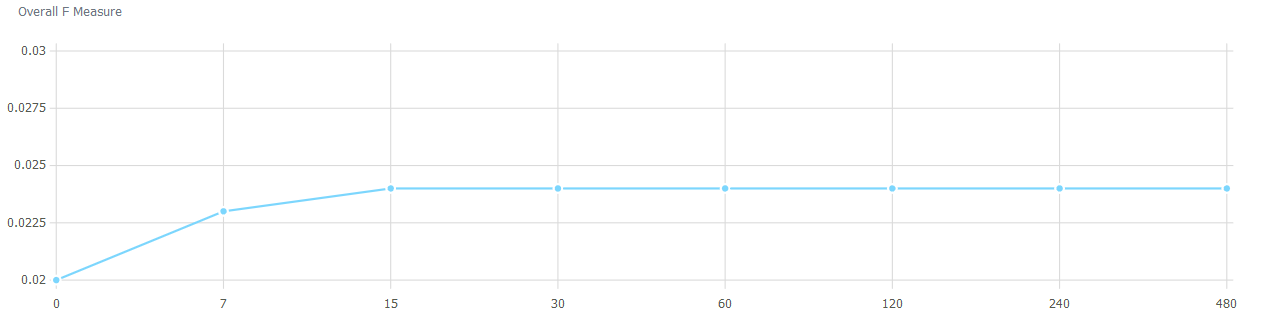
\includegraphics[width=\linewidth]{images/1day-merged-f-measure.png}
		      \caption{1 Day Merged - F-Measure}
		      \label{fig:1day-merged-f-measure}
		  \end{figure}
		  
		  Similar results were registered for the 7-day data set. \\
		  The overall f-measure had increased from its baseline value, to a high of 0.36 for window values of 240 and 480 minutes.
		  Interestingly enough, the events detected by the evaluation script had increased as well, from 106 baseline to 112.
		  \\
		  Moreover, recall followed the trend set by the 1-day dataset and increased from 0.209 initially to 0.221 for window of 240 and 480 minutes respectively. 
		  The number of clusters had steadily decreased as the window grew, which was expected behaviour.
		  As a result, the precision measure of the system had grown as well.
	      \begin{figure}[h!]
		      \centering
		      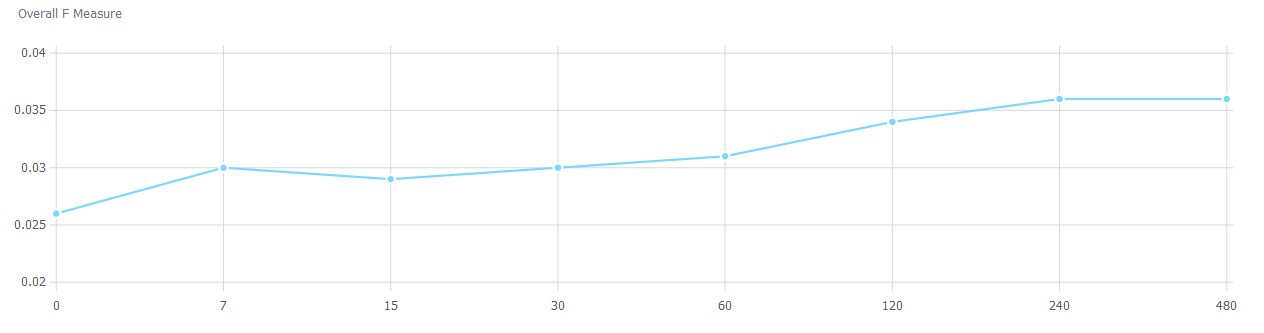
\includegraphics[width=\linewidth]{images/7days-merged-f-measure.png}
		      \caption{7 Days Merged - F-Measure}
		      \label{fig:7days-merged-f-measure}
	      \end{figure}
\end{enumerate}

%%%%%%%%%%%%%%%%%%%%%%%%%%%%%%%%%%%%%%%%%%%%%%%%%%%%%%%%%%%%%%%%%%%%%%%%%%%%%%%%%%
\section{Discussion}
\label{section-discussion}

The summary of the results can be seen in Figure \ref{fig:summary}.
The table shows the baseline results, along with the results with the highest f-measures of the two approaches applied on both data sets.\\
\\
From the results, there were a few interesting conclusions drawn. 
The first, was that the filtering step enhanced the cluster identification step from McMinn's study \cite{McMinn2013} and greatly increased the evaluation results without any impact on the recall.
This can be said for both data sets.
As a result of the filtering process, the precision skyrocketed along with the f-measure by an order of magnitude. \\
In terms of scalability, this step could be easily implemented on a stream of clusters as it is simply a case of pass/drop by comparing sizes.
However, one must be careful when choosing the scalar to sort by.
Relevant clusters might easily be dropped if not handled carefully and thus might have a negative impact on recall.

\begin{figure}[h!]
	\centering
	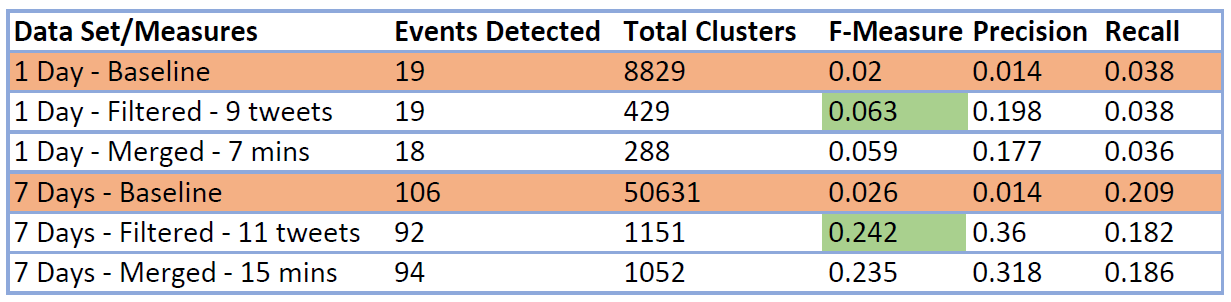
\includegraphics[width=\linewidth]{images/summary.png}
	\caption{Summary of results}
	\label{fig:summary}
\end{figure}

By contrast, the merging approach did not attain the same highs.
Still, the results were surprising since recall was not expected to increase further than the baseline.
This might be due to the increase in the number of events detected which increased by a few values (by 1 in the 1-day dataset, by 6 in 7-day).
As a result, this step might be considered an enhancement of the clustering step, where multiple clusters with the same named entity was created. 
Such behaviour might be expected in the case where users tweeted later than the time of event occurence and selected clustering window being too small.
\\\\
In theory, it should be an unharmful operation provided there are no other clusters with the same named entity in the same temporal window.
Additionally, it would be interesting to find what the results could be with the filtering step applied before the merge.
In theory, it should get rid of the small clusters with no relevance to an event and dramatically decrease the size of the output. 
Still, as mentioned earlier, care must be taken with the variable on which to filter on.
\\
However, there could be a major setbacks to the merging of same named entity clusters.
A possible worst case would be in the case where two or more events occurred within minutes of each other, all related to the same entity, but considered as two different events. 
This approach would fail at picking up all the events and, instead, returning only a single one. 
\\\\
Finally, both approaches provide an enhacement for event detection provided by McMinn's \cite{McMinn2013}.
However, it is arguable whether they could be used in real-time systems.
Filtering clusters in real-time is challenging, since it would be difficult to say what is relevant and what is not purely based on number of tweets in a current cluster.
Merging of selected clusters might provide more concise data through merging events with the same entity, but would fail in the case where two events with the same entity occurred in the same temporal space.

%%%%%%%%%%%%%%%%%%%%%%%%%%%%%%%%%%%%%%%%%%%%%%%%%%%%%%%%%%%%%%%%%%%%%%%%%%%%%%%%%%
\section{Traffic Event Detection}
\subsection{Problem Statement}

Traffic blockages and congestions are more and more important in the daily lives of commuters, public transport drivers and for the general "health" of the city.
In the UK alone, the average commuter would spend 32 hours on in traffic each year and drivers spend an additional 9\% of their time driving as per the INRIX Scorecard for UK 2016 \cite{INRIXdata}. 

Efficient solutions to traffic problems are still to be found.
An interesting idea, provided by Elon Musk's company, named ironically \textit{The Boring Company}, is to create tunnels under the city in order to reduce congestion in the city of Los Angeles.
This idea came through due to Elon's time wasted in traffic, as per his interview \cite{ElonTED}.

However, there is a need to find an alternative and more efficient solution rather than digging holes in the ground.
This is where social media data provides an alternative for a cheap and efficient way to share traffic information.
If accidents, congestions, traffic issues could be reported via Twitter.
A social media platform, such as Twitter, already provides up-to-date real-time information and this data could be used for trafic analysis.

Nevertheless, the issues with Twitter remain, as mentioned before, as well as:
\begin{itemize}
	\item Geo-tagging. Only 10\% of daily tweets are geo-tagged. For a traffic analysis solution to work consistenly, geo-location is a must.
	However, if no such data is provided, there must be a method for extracting valuable data from the body text and complete the geographical information issue.
	\item Temporality. It is important that tweets are grouped according to time. 
	Most up-to-date information is essential for avoiding the increase of congestion.
	\item Trust. Information must be relevant either by coming from multiple sources or by analysis of trusted sources.
	An example of a trusted source is Transport For London (TFL), which posts hourly updates on its Twitter account.    
\end{itemize}


%==============================================annotated bibliography
\newpage
\nocite{*}
\bibliographystyle{plain}
\bibliography{bibliography}
\pagebreak

% Activate the appendix
% from now on sections are numerated with capital letters
\appendix

%%%%%%%%%%%%%%%%%%%%%%%%%%%%%%%%%%%%%%%%%%%%%%%%%%%%%%%%%%%%%%%%%%%%%%%%%%%%%%%%%%
\section{Experiment Results}
\label{appendix:results}

\subsection{1-day Data-Set}
\subsubsection{Filtering}

\begin{figure}[H]
	\centering
	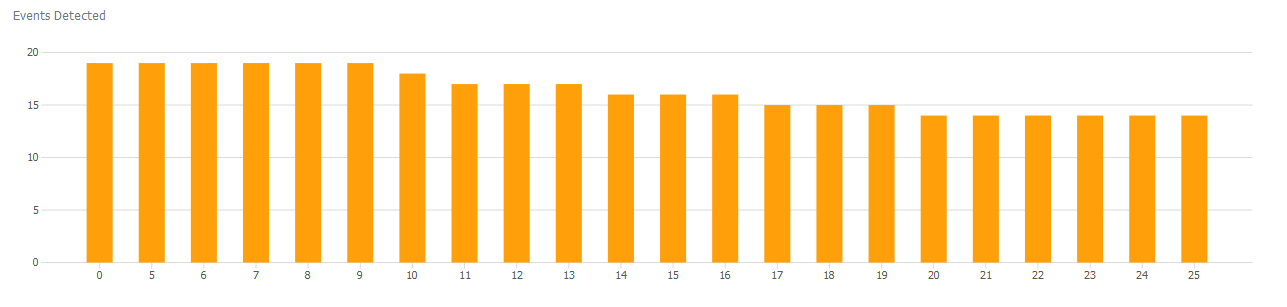
\includegraphics[width=\linewidth]{images/1day-filtered-events-detected.png}
	\caption{1-Day Filtered Events Detected}
	\label{fig:1day-filtered-events-detected}
\end{figure}

\begin{figure}[H]
	\centering
	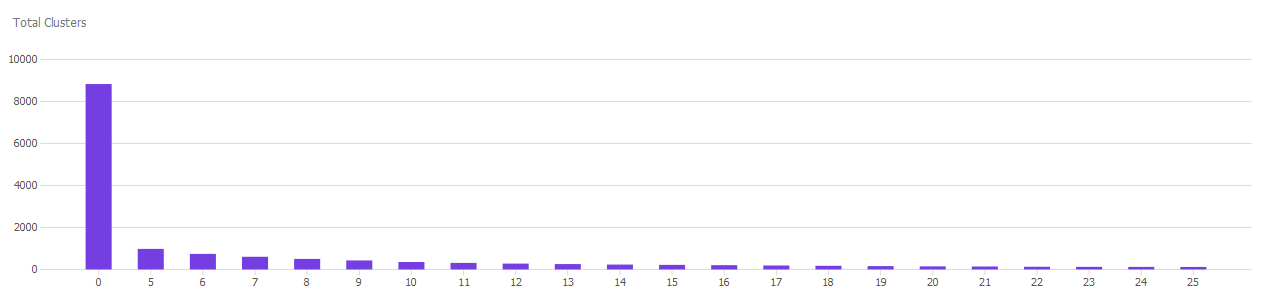
\includegraphics[width=\linewidth]{images/1day-filtered-total-clusters.png}
	\caption{1-Day Filtered Total Clusters}
	\label{fig:1day-filtered-total-clusters}
\end{figure}

\begin{figure}[H]
	\centering
	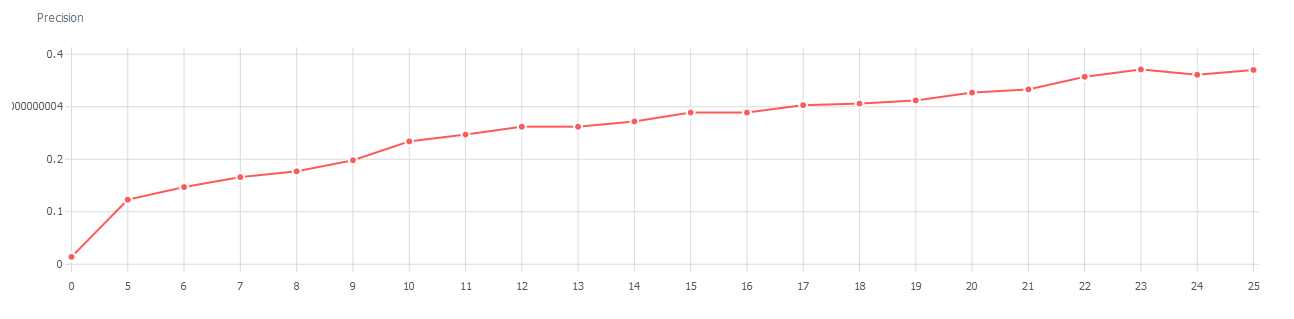
\includegraphics[width=\linewidth]{images/1day-filtered-precision.png}
	\caption{1-Day Filtered Precision}
	\label{fig:1day-filtered-precision}
\end{figure}

\begin{figure}[]
	\centering
	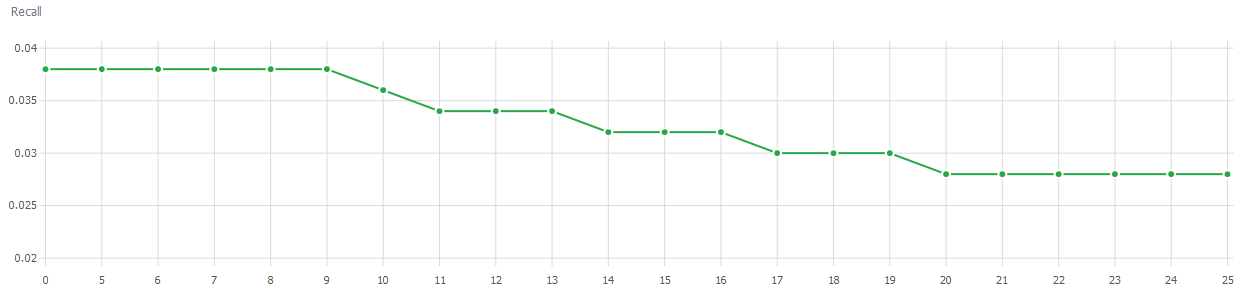
\includegraphics[width=\linewidth]{images/1day-filtered-recall.png}
	\caption{1-Day Filtered Recall}
	\label{fig:1day-filtered-recall}
\end{figure}

\begin{figure}[H]
	\centering
	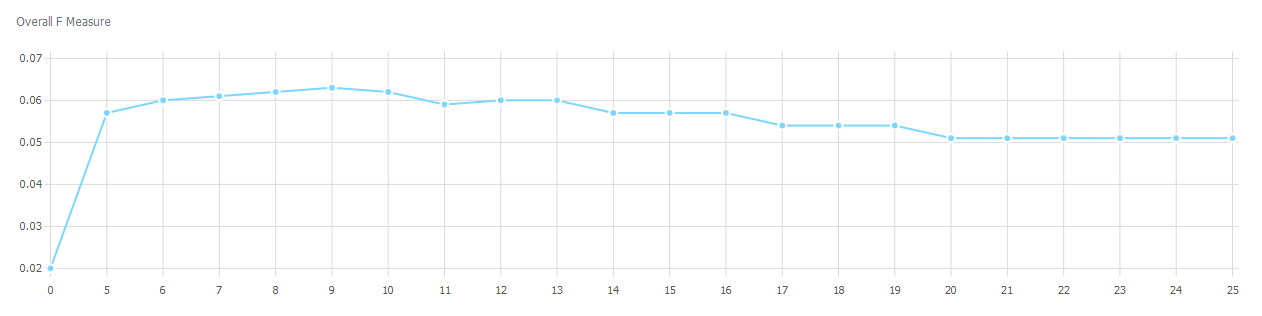
\includegraphics[width=\linewidth]{images/1day-filtered-f-measure.png}
	\caption{1-Day Filtered F-Measure}
	\label{fig:1day-filtered-f-measure}
\end{figure}

\subsubsection{Merging}

\begin{figure}[H]
	\centering
	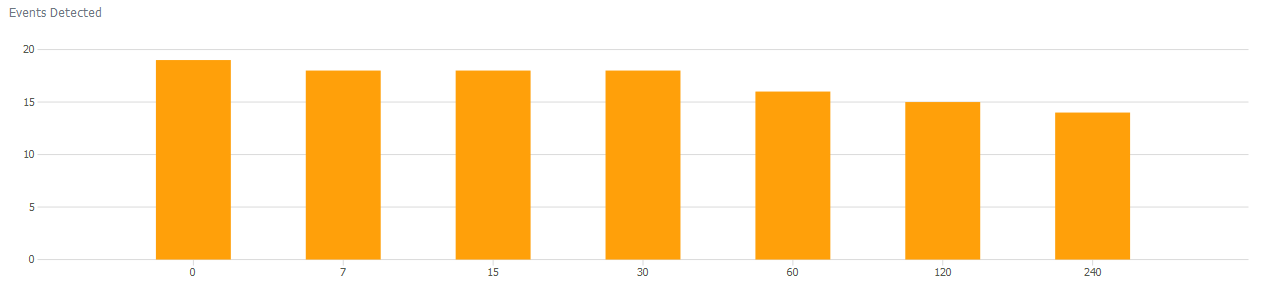
\includegraphics[width=\linewidth]{images/1day-merged-events-detected.png}
	\caption{1-Day Merged Events Detected}
	\label{fig:1day-merged-events-detected}
\end{figure}

\begin{figure}[H]
	\centering
	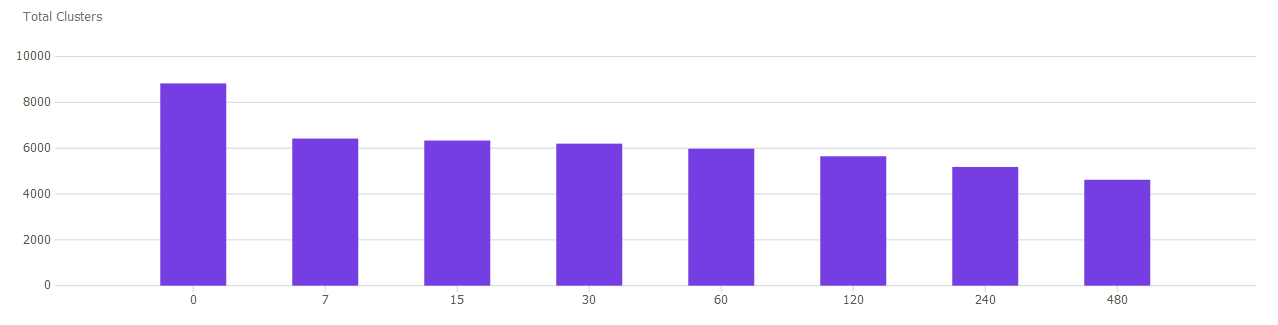
\includegraphics[width=\linewidth]{images/1day-merged-total-clusters.png}
	\caption{1-Day Merged Total Clusters}
	\label{fig:1day-merged-total-clusters}
\end{figure}

\begin{figure}[H]
	\centering
	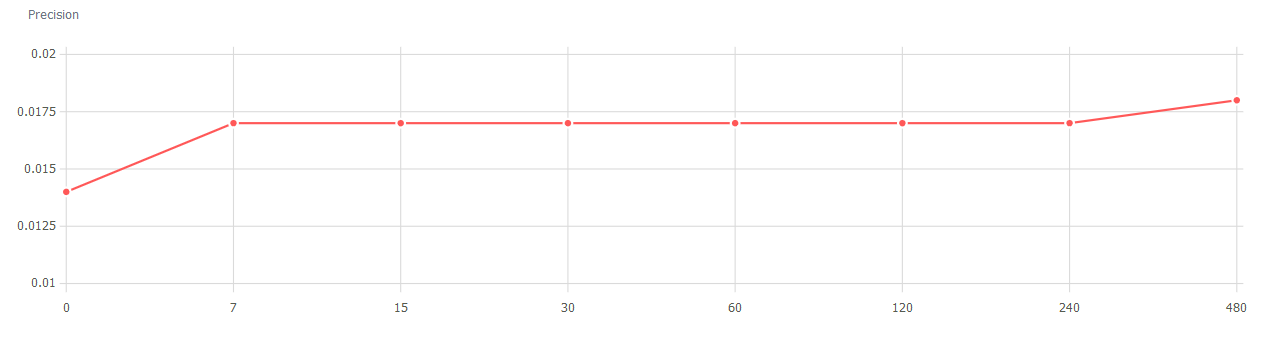
\includegraphics[width=\linewidth]{images/1day-merged-precision.png}
	\caption{1-Day Merged Precision}
	\label{fig:1day-merged-precision}
\end{figure}

\begin{figure}[H]
	\centering
	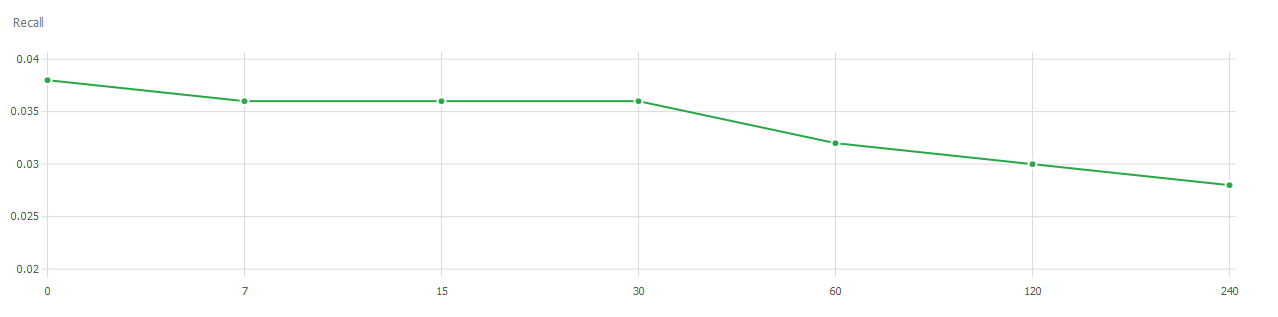
\includegraphics[width=\linewidth]{images/1day-merged-recall.png}
	\caption{1-Day Merged Recall}
	\label{fig:1day-merged-recall}
\end{figure}

\begin{figure}[H]
	\centering
	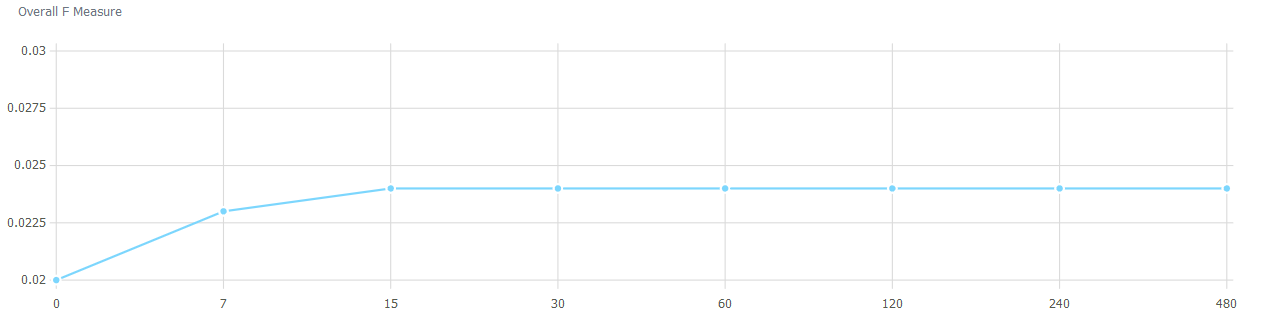
\includegraphics[width=\linewidth]{images/1day-merged-f-measure.png}
	\caption{1-Day Merged F-Measure}
	\label{fig:1day-merged-f-measure}
\end{figure}

%%%%%%%%%%%%%%%%%%%%%%%%%%%%%%%%%%%%%%%%%%%%%%%%%%%%%%%%%%%%%%%%%%%%%%%%%%%%%%%%%%
\subsection{7-day Data-Set}
\subsubsection{Filtering}

\begin{figure}[H]
	\centering
	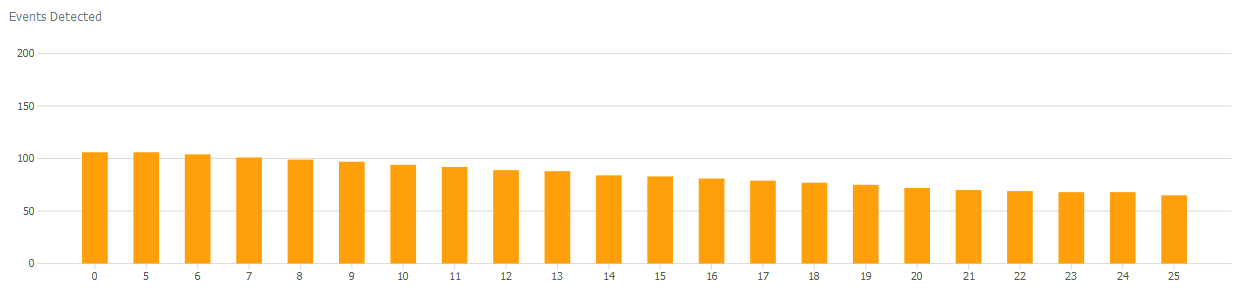
\includegraphics[width=\linewidth]{images/7days-filtered-events-detected.png}
	\caption{7-Day Filtered Events Detected}
	\label{fig:7day-filtered-events-detected}
\end{figure}

\begin{figure}[H]
	\centering
	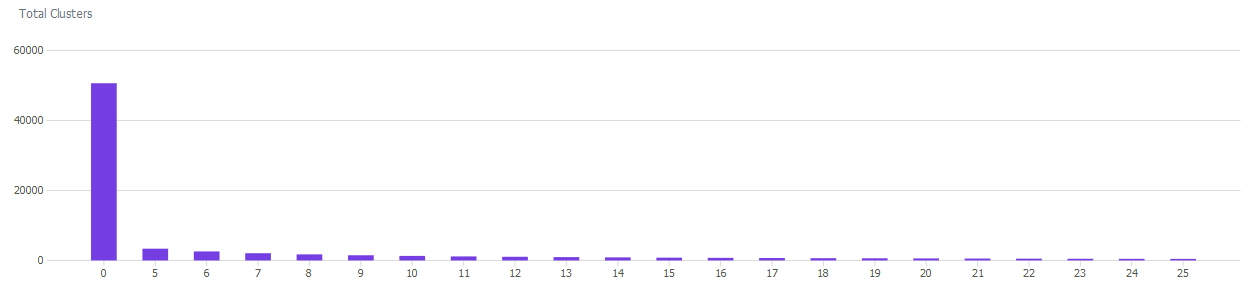
\includegraphics[width=\linewidth]{images/7days-filtered-total-clusters.png}
	\caption{7-Day Filtered Total Clusters}
	\label{fig:7days-filtered-total-clusters}
\end{figure}

\begin{figure}[H]
	\centering
	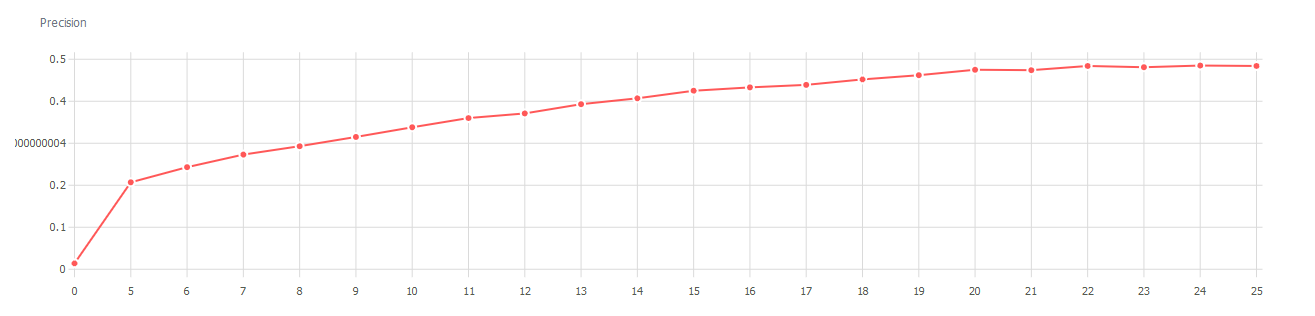
\includegraphics[width=\linewidth]{images/7days-filtered-precision.png}
	\caption{7-Day Filtered Precision}
	\label{fig:7days-filtered-precision}
\end{figure}

\begin{figure}[H]
	\centering
	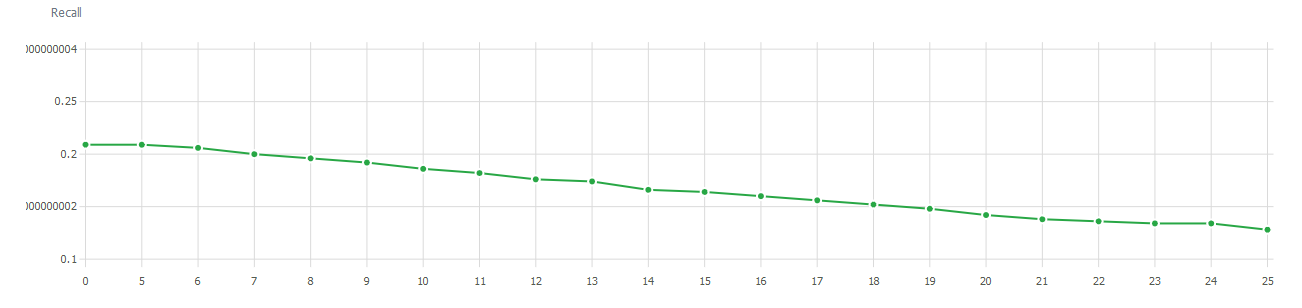
\includegraphics[width=\linewidth]{images/7days-filtered-recall.png}
	\caption{7-Day Filtered Recall}
	\label{fig:7days-filtered-recall}
\end{figure}

\begin{figure}[H]
	\centering
	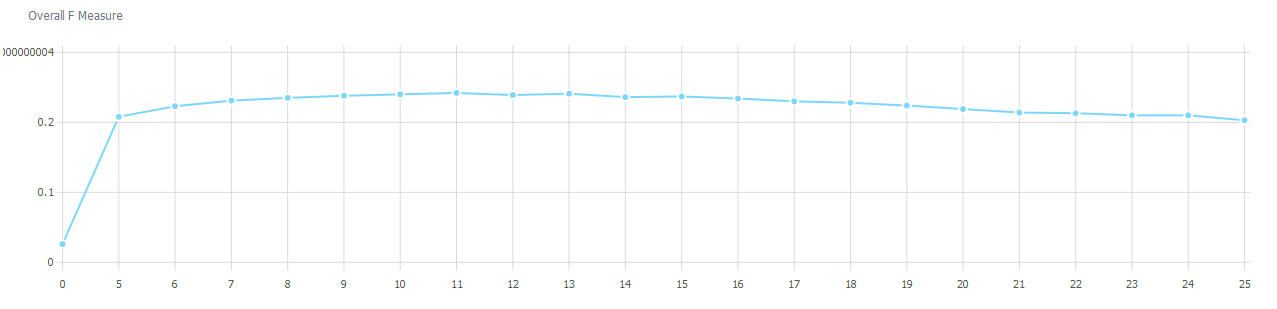
\includegraphics[width=\linewidth]{images/7days-filtered-f-measure.png}
	\caption{7-Day Filtered F-Measure}
	\label{fig:7days-filtered-f-measure}
\end{figure}

\subsubsection{Merging}

\begin{figure}[H]
	\centering
	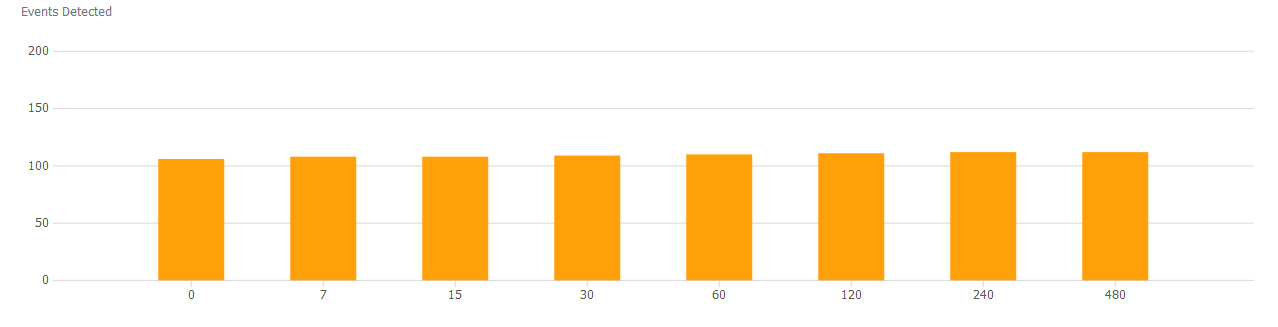
\includegraphics[width=\linewidth]{images/7days-merged-events-detected.png}
	\caption{1-Day Merged Events Detected}
	\label{fig:7days-merged-events-detected}
\end{figure}

\begin{figure}[H]
	\centering
	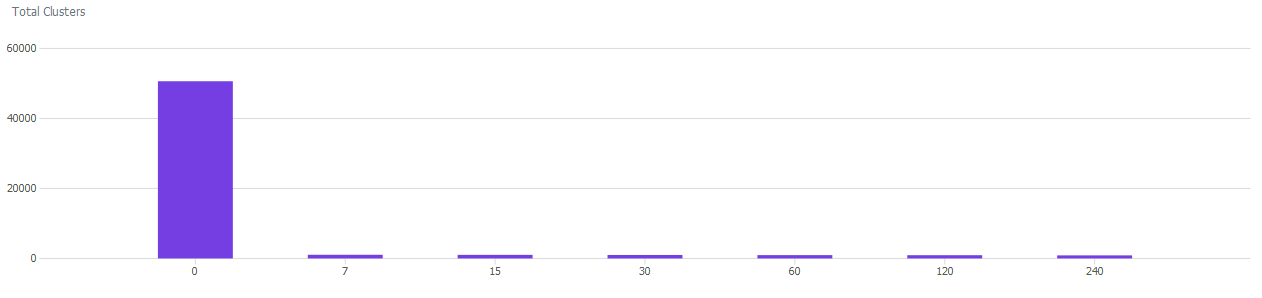
\includegraphics[width=\linewidth]{images/7days-merged-total-clusters.png}
	\caption{1-Day Merged Total Clusters}
	\label{fig:7days-merged-total-clusters}
\end{figure}

\begin{figure}[H]
	\centering
	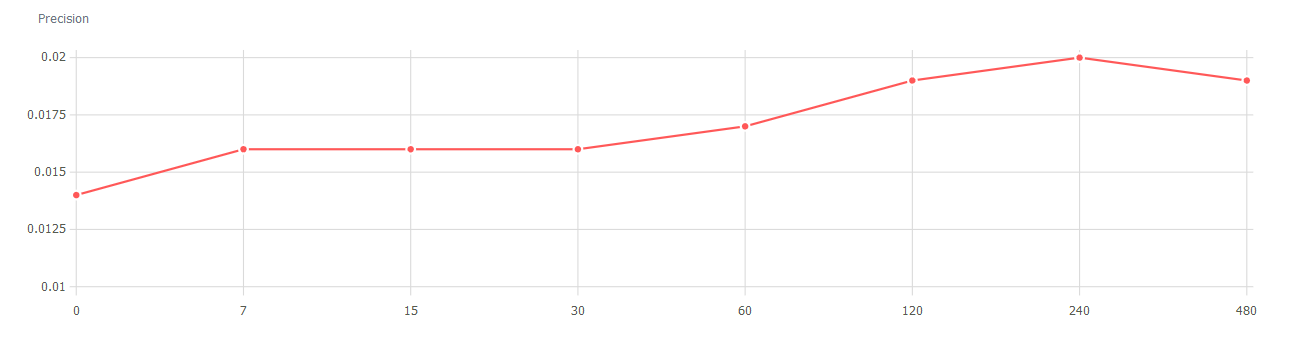
\includegraphics[width=\linewidth]{images/7days-merged-precision.png}
	\caption{1-Day Merged Precision}
	\label{fig:7days-merged-precision}
\end{figure}

\begin{figure}[H]
	\centering
	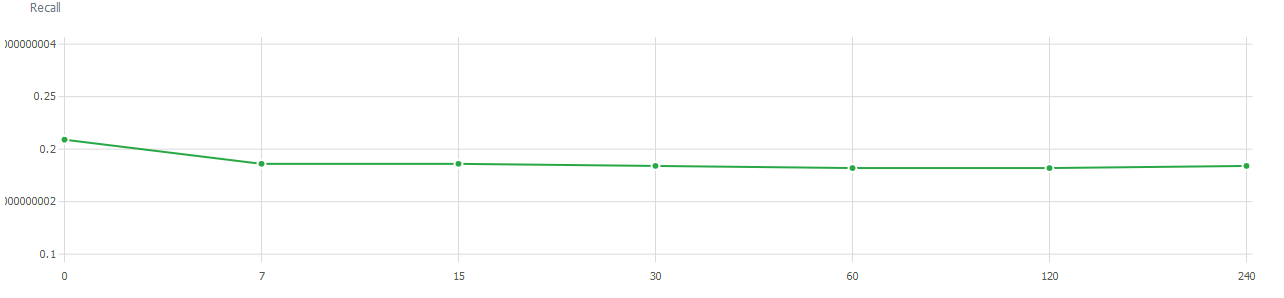
\includegraphics[width=\linewidth]{images/7days-merged-recall.png}
	\caption{1-Day Merged Recall}
	\label{fig:7days-merged-recall}
\end{figure}

\begin{figure}[H]
	\centering
	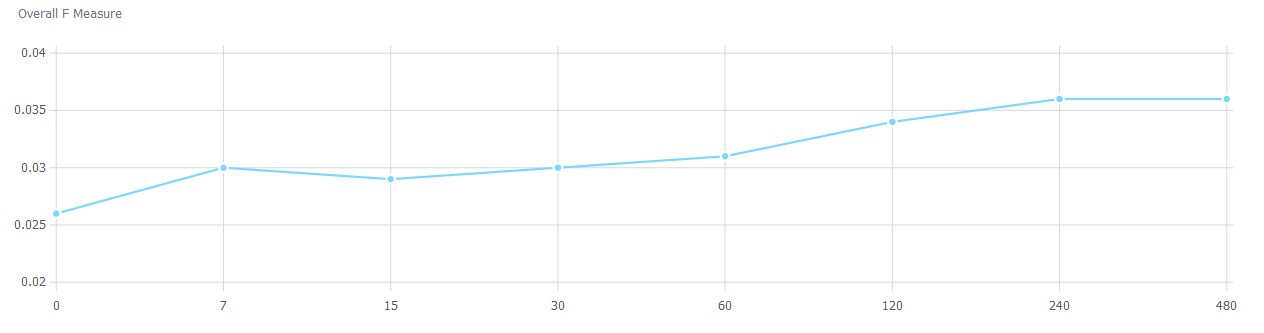
\includegraphics[width=\linewidth]{images/7days-merged-f-measure.png}
	\caption{1-Day Merged F-Measure}
	\label{fig:7days-merged-f-measure}
\end{figure}


\end{document}
